%%% Use the next line if you want questions
\documentclass[12pt,addpoints]{exam}
%%% OR, use the next line if you want solutions
%\documentclass[12pt,answers,addpoints]{exam}



\usepackage{amsmath}
\usepackage{graphicx}
\begin{document}

%% Some Formatting Options:
%% Make an easy blank environment (just type \blank{1.5in} now)
\newcommand\blank[1]{\makebox[#1]{\hrulefill}}
%% Tell TeX to make linebreaks before questions begin
\newcommand{\myquestion}{\filbreak\question}
\newcommand{\mypart}{\filbreak\part}
%% then replace all your \question commands with \myquestion
%% commands.  \filbreak basically means "this is a good place to break
%% the page, and fill the bottom of the page with blank space, unless you
%% can put enough more on the page to reach the next \filbreak, in which
%% case the present \filbreak will have no effect at all".  The effect of
%% \filbreak before each question is that page breaks will occur only
%% before questions.
%% This command below makes an even nicer fill-in-the-blank.
\newcommand*{\TickBox}{{\fboxsep 0pt \fbox{\rule{0em}{2em}\rule{10em}{0em}}}}

\begin{coverpages}

\begin{center}
\begin{Large}
\vspace{-0.3in}
A Sample Exam in \LaTeX 
\end{Large}
\end{center}

\vspace{0.5in}

\begin{center} \fbox{\fbox{\parbox{5.5in}{

The exam consists of \numpages{} pages, not including this cover page.  Please go
through your copy to make sure that all pages have been printed.

\bigskip

The
first part of the exam consists of short questions.  No partial credit will be
given.  The second part of the exam consists of longer questions.  Partial
credit will be given for correct reasoning.  Show all work for the longer
questions.  There are \numpoints{} points, total, on this exam.

\bigskip

Good luck!
}}}
\end{center}

\vspace{0.8in}
\makebox[\textwidth]{Name:\enspace\hrulefill}

\vspace{0.3in}

\makebox[\textwidth]{ID Number:\enspace\hrulefill}

\vspace{1.1in}

\begin{center}
\begin{small}
\gradetable[v][pages] 
\end{small}
\end{center}


\end{coverpages}

\pagestyle{headandfoot} \extraheadheight{.25in} 
\firstpageheader{} {My University\\ This Semester \\ Final Examination \\ Economics 101} {} 
\footer{} {Page \thepage\ of \numpages} {\iflastpage{End of exam.}{Please go on to the next page\ldots}}



\begin{questions}
\fullwidth{\Large \textbf{Short Questions}} 

\uplevel{No partial credit will be awarded.  Clearly circle \emph{one} choice
for each of the multiple-choice questions.  }

\myquestion[5] A small coffee company roasts coffee beans in its shop. 
The {\em total} cost of roasting coffee beans is $3q^2$ when
$q$ pounds are roasted. 
The smell of roasting beans imposes costs on the 
company's neighbors. The {\em total} amount that neighbors 
would be willing to pay to have the shop stop roasting 
altogether is $\frac{3}{2} \cdot q^2$. The company sells its output in a 
competitive market at \$36 per pound, so that its total revenue is $36q$. What is the 
socially efficient amount of coffee for the company to 
roast? 
	\begin{choices}
	\choice 2 pounds. 
	\CorrectChoice 4 pounds.
	\choice 6 pounds.
	\choice 8 pounds.
	\choice 10 pounds.
	\end{choices}

\myquestion[5] A monopolist has discovered that the inverse demand function of a
person with income M for the monopolist’s product is $p = 0.002M - q$. The
monopolist is able to observe the incomes of its consumers and to practice price
discrimination according to income.
 The monopolist has a total cost function, $c(q) = 100q$. The
price it will charge a consumer depends on the consumer's income, $M$, according
to the formula
	\begin{choices}
	\choice $p = 0.002M - 100$
	\choice $p = M^2$
	\choice $p = 0.01 M^2 + 100$
	\CorrectChoice $p = 0.001M + 50$
	\choice None of the above.
	\end{choices}

\myquestion[5] An industry consists of two duopolist firms choosing their output
simultaneously.  They decide to enter into a secret agreement to maximize their
joint profits.  The {\em total} output of the industry then goes $[X]$ and the
price goes $[Y]$.
	\begin{choices}
	\choice $X =$ up, $Y =$ down
	\choice $X =$ up, $Y =$ up
	\choice $X =$ stays the same, $Y =$ up
	\choice $X =$ down, $Y =$ down
	\CorrectChoice $X =$ down, $Y =$ up
	\end{choices}

\uplevel{The following two questions refer to the figure below.  The figure depicts cost
curves for a firm.  To answer the questions, simply refer to points labeled by
capital letters on the graph.}

\begin{center}
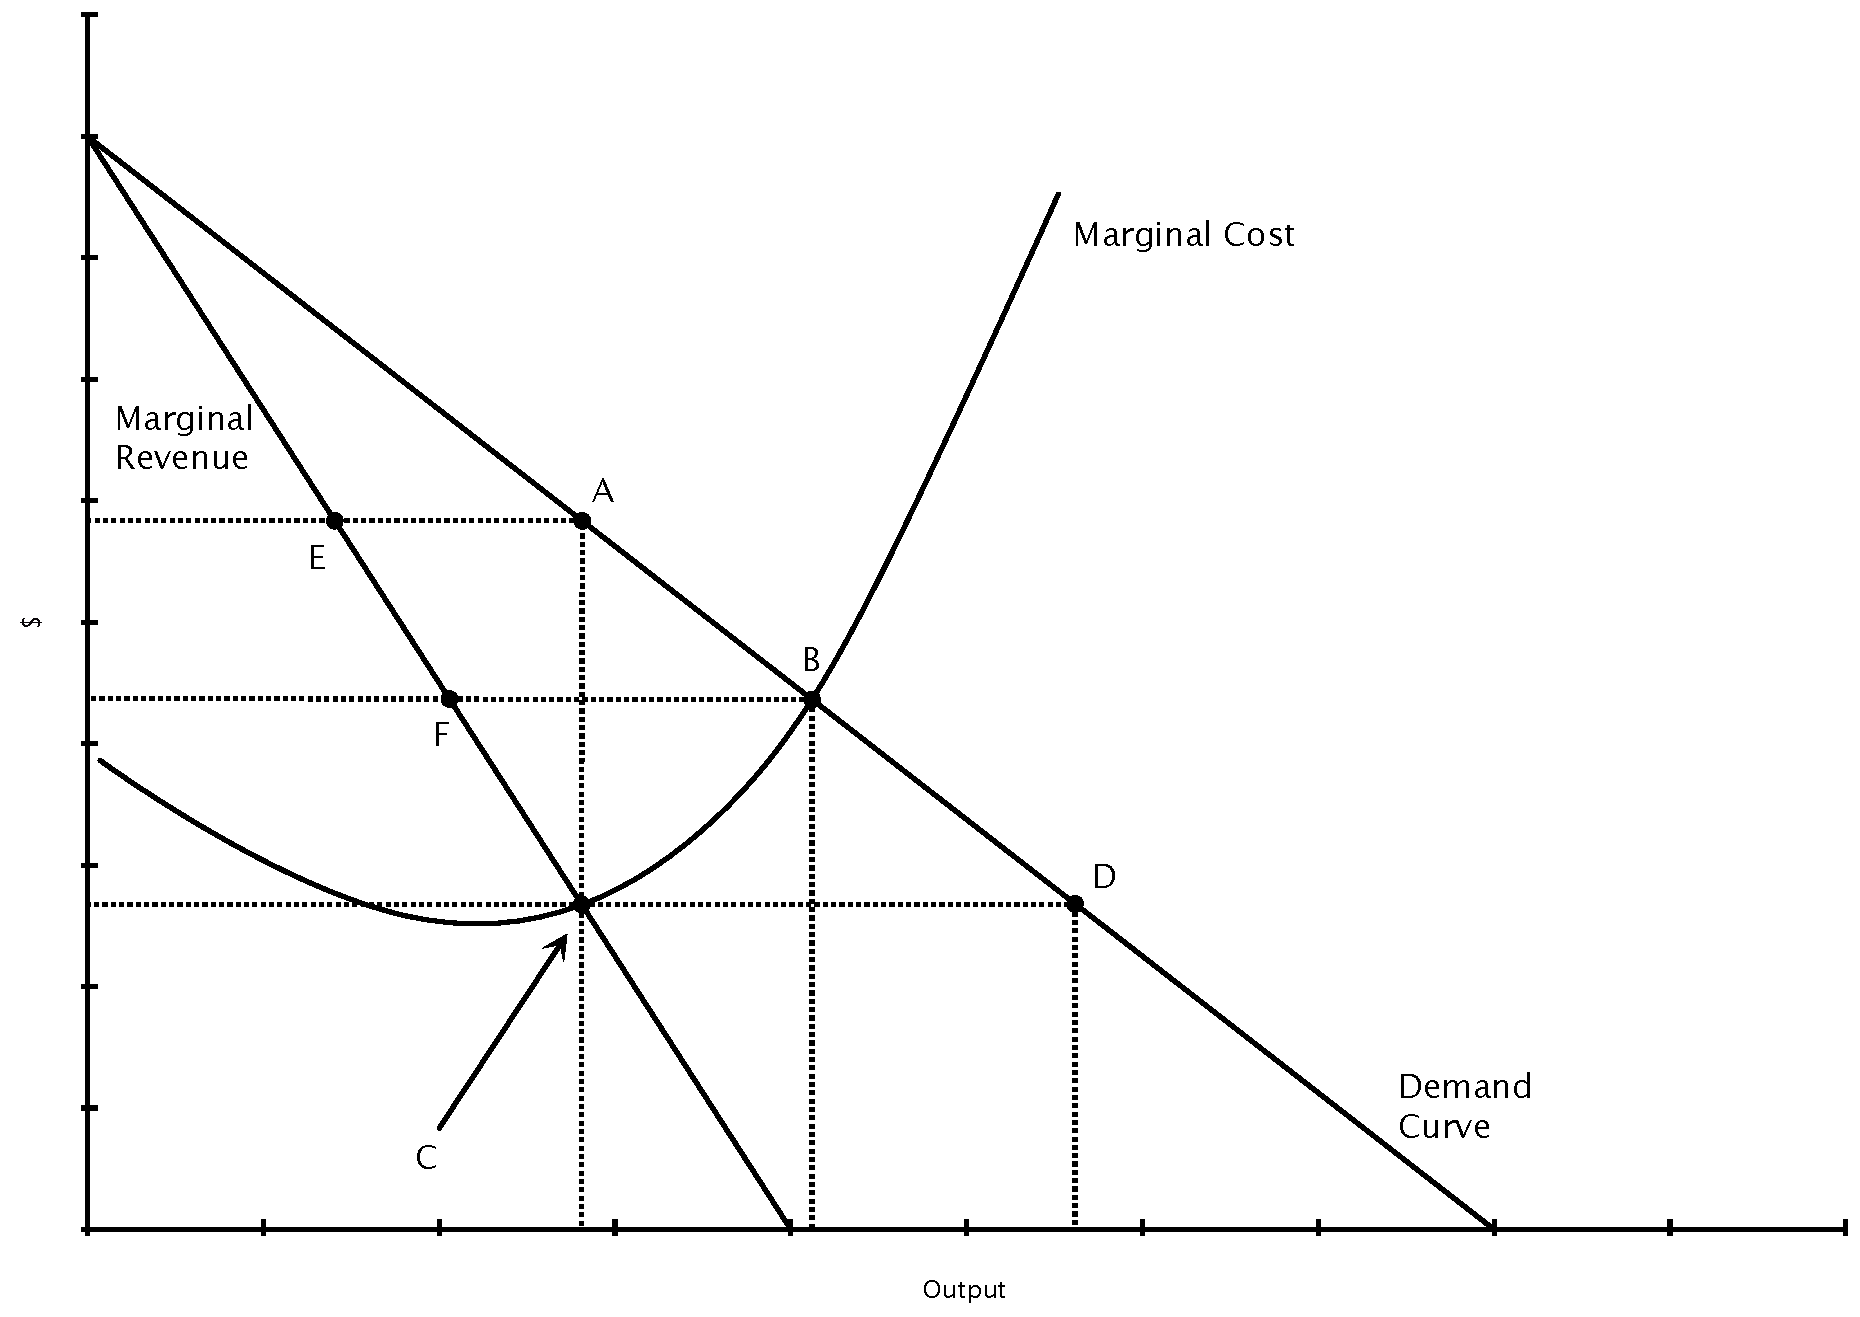
\includegraphics[scale=.43]{fig1.pdf}
\end{center}

\myquestion[5] If the firm behaves competitively, taking price as given, what
level of output and price does it choose?
	\answerline

	\begin{solution}
	Bundle $B$.
	\end{solution}

\myquestion[5] If the firm acts as a monopolist, what level of output and price
does it choose?
	\answerline 

	\begin{solution}
	Bundle $A$.
	\end{solution}

\myquestion[5] Suppose that a consumer considers coffee ($C$) and tea ($T$) to be perfect substitutes, but he
requires two cups of tea to give up one cup of coffee. This consumer's budget constraint
can be written as $2.5C + T = 10$. What should the consumer buy?
	\begin{choices}
	\choice 2 cups of tea and no coffee.
	\CorrectChoice 10 cups of tea and no coffee
	\choice 2.5 cups of coffee and no tea.
	\choice 4 cups of coffee and no tea.
	\choice none of the above.
	\end{choices}

\myquestion[5] The market demand curve is $D\left( p \right) = 20 - 16\cdot p$.  When
the price is \$1, what is the elasticity of demand?
\answerline

	\begin{solution}
	First, we calculate the elasticity of demand using the usual formula:
	$$ \frac{\partial D(p)}{\partial p} \cdot \frac{p}{D(p)} = 
	-16 \cdot \frac{p}{20 - 16p}.$$
	If we plug in $p=1$, we find that the elasticity of demand is $-16 \cdot
	\frac{1}{20-16} = -4$.
	\end{solution}

%%%%%%%%%%
%%%%%%%%%%
%%%%%%%%%%
%%%%%%%%%%
%%%%%%%%%%

\newpage
\fullwidth{\Large \textbf{Problems}} 

\uplevel{For the following problems, show all your work.  Partial
credit will be awarded for correct reasoning.   }

\question Suppose that a consumer likes apples ($a$)
and bananas ($b$), and has utility function $u\left(a,\,
b\right)=a^{2/10} \cdot b^{8/10}$.
Suppose that apples cost \$10 a pound and that the consumer has \$100
to spend. Denote the price of bananas as $p$. 
	\begin{parts}
	\part[5] What is the consumer's budget constraint?

	\begin{solution}[2.5in]
	The consumer's budget constraint is $10a+pb\leq100$. 
	\end{solution}

	\part[5] What is the consumer's marginal rate of substitution. In 1--2
	sentences describe what this quantity represents, aside from just ``the
	slope of the indifference curve.''
	\begin{solution}[2.5in]
	The consumer's marginal rate of substitution is \[ -\frac{\partial
	u/\partial a}{\partial u/\partial b}=-\frac{\left(2/10\right)\cdot
	a^{-8/10}\cdot b^{8/10}}{\left(8/10\right)\cdot a^{2/10}\cdot
	b^{-2/10}}=-\frac{2}{8}\cdot\frac{b}{a}.\] Note that this {}``assumes''
	we're graphing apples on the horizontal axis.
	\end{solution}
	
	\clearpage

	\part[5] Setting the MRS equal to the slope of the budget constraint, find
	the consumer's optimal choice of apples in terms of bananas.

	\begin{solution}[3in]
	If we graph apples on the horizontal axis, then the MRS is as above,
	and the slope of the budget constraint is $-10/p$. So at the consumer's
	utility-maximizing choice of goods, we must have\[
	\frac{10}{p}=\frac{2}{8}\cdot\frac{b}{a},\]
	which in turn implies that $a^{*}=\frac{2p}{80}\cdot b$.
	\end{solution}

	\part[5] Plug this result into the budget constraint to find the consumer's
	demand for bananas.

	\begin{solution}[3in]
	Plugging in, we have\[
	10\cdot\frac{2p}{80}\cdot b+pb=100,\]
	which implies that \[
	b^{*}=\frac{100}{p\cdot\left(\frac{20}{80}+1\right)}=\frac{80}{p}.\]
	\end{solution}

\end{parts}

\myquestion Suppose that a competitive firm has production function $f\left(K,L\right)=\sqrt{KL}$,
in which $K$ denotes capital and $L$ denotes units of labor. The
firm must pay its workers sixteen dollars an hour, and must pay $r$
dollars per unit of capital. 
	\begin{parts}
	\part[5] Does the firm have constant, increasing, or decreasing returns to
	scale? Justify your answer.

	\begin{solution}[2in]
	Constant returns to scale: \[ f\left(2K,\,2L\right)=\sqrt{2\cdot
	K\cdot2\cdot L}=2\sqrt{K\cdot L}=2\cdot f\left(K,\, L\right).\]
	\end{solution}

	\part[5] Calculate the firm's technical rate of substitution (TRS). In
	1--2 sentences, describe what this quantity represents, aside from just
	{}``the slope of the isoquant.''

	\begin{solution}[2in]
	The firm's technical rate of substitution is \[ \frac{\partial
	f\left(K,\, L\right)/\partial K}{\partial f\left(K,\, L\right)/\partial
	L}=\frac{\frac{1}{2}K^{-0.5}L^{0.5}}{\frac{1}{2}\cdot
	K^{0.5}L^{-0.5}}=\frac{L}{K}.\] Note this assumes that capital is on the
	horizontal axis. 
	
	The TRS measures the firm's ability to substitute
	capital for labor while holding output constant.
	\end{solution}

	\part[5] Find the firm's conditional
	demand for labor, $L^{*}\left(r,y\right)$ in terms of the price
	of capital and the firm's choice of output.  (Hint: set the TRS equal to
	the slope of an iso-cost curve, and solve for capital in terms of labor.
	Then plug that result into the production function.)

	\begin{solution}
	The firm's iso-cost line is $C=16L+rK$. If capital is on the horizontal
	axis, then $L=\frac{C}{16}-\frac{r}{16}K$. So at the optimum level
	of inputs, we observe\[
	\frac{r}{16}=\frac{L}{K}.\]
	This implies that $K=\frac{16L}{r}$. Plugging this into the production
	function leads to $y=\sqrt{\frac{16L}{r}\cdot L}=4L\cdot r^{-1/2}$.
	So the conditional demand curve for labor is \[
	L^{*}=\frac{y}{4}\cdot\sqrt{r}.\]
	\end{solution}
	 
	\end{parts}


\end{questions}


\end{document}
